\chapter{The Twitter potential reach of FET projects on quantum technologies}
As shown in chapter \ref{FET_projects_and_social_media}, FET research projects on QT make limited use of online communication channels. In particular, none of them has considered the creation of an account on Twitter, the most common social platform among FET initiatives. It is therefore interesting to assess the broadness of the community which could be reached by QT projects via Twitter.

To this aim, the following analysis was performed. First, one hashtag likely to be mentioned in QT-related tweets was chosen. The hashtag was then monitored over two periods of time. The same procedure was repeated for one hashtag representative of mentions on HPC. The comparison of the outcomes of the two monitoring procedures provided an estimate of the communication potential of FET QT projects via Twitter. The monitoring activities were performed with the Twitter Analytics Tool Twitonomy. The Twitonomy application was also used to obtain all plots in this chapter.

\begin{figure}[!t] 
 \begin{center}
 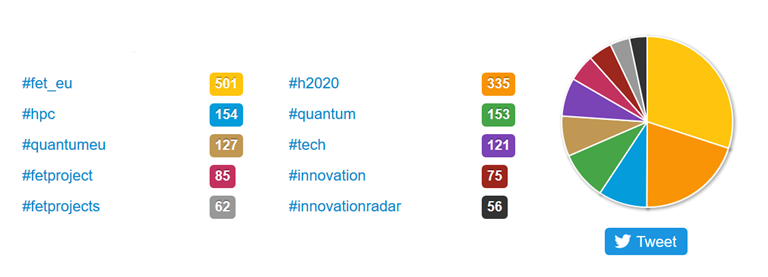
\includegraphics[scale=0.58]{Images/Hashtags_feteu.png}
 \caption{Most used hashtags of the Twitter profile @fet\textunderscore eu of the FET funding programme. The values refer to the 3 199 tweets posted by the account between 8 January 2016 and 25 October 2017. HPC- and QT-related hashtags are the first in the ranking among scientific keywords.}
 \label{Hashtags_feteu}
 \end{center}
\end{figure}

HPC was chosen as a suitable class for comparison for the following reasons: \textit{i}) HPC and QTs are among the most important topics in FET communication, see figure \ref{Hashtags_feteu}; \textit{ii}) HPC projects are active initiatives within the FET community in terms of online communication; \textit{iii}) HPC and QT projects share similar communication challenges, see section \ref{Online_presence_breakdown}.

This chapter is structured as follows. Sections \ref{Monitoring_of_the_QT_hashtag} and \ref{Monitoring_of_the_HPC_hashtag} outline the monitoring activity launched for the QT and HPC hashtags. The comparison of the results and the assessment of the Twitter potential community of FET QT projects are reported in section \ref{Comparison_of_the_results}. 

\section{Monitoring of the QT hashtag} \label{Monitoring_of_the_QT_hashtag}
The QT hashtag monitored for the analysis presented in this chapter was \#quantumcomputing. The hashtag was chosen for the relevance of quantum computers in QT research, see section \ref{FET_and_quantum_technologies}. 

\begin{table}[t]
 \begin{center}
  \begin{tabular}{cccc}
   \hline 
   \hline
   Time period & Tweets & Users & Potential Reach \\ 
   \hline
   \hline
   7 - 14 Oct 2017 & 1 928 & 1 270 & 9 392 166  \\
   20 - 25 Oct 2017 & 2 563 & 1 738 & 10 604 445  \\
   \hline
   \hline
  \end{tabular}
 \end{center} 
 \caption{Statistics calculated for the mentions on Twitter of the hashtag \#quantumcomputing over the monitored time periods. The potential reach is defined as the total aggregate number of followers of the accounts which mentioned the considered keyword in their tweets.}
\label{Summary_QuantumComputing} 
\end{table}

The monitoring activity covered two periods of time: from 7 to 14 and from 20 to 25 October 2017, respectively. The time periods were chosen randomly and based on the amount of mentions which could be tracked by Twitonomy. Different choices of the time periods would not change the order of magnitude of the estimates presented in this chapter.

\begin{figure}
 \centering
 \begin{subfigure}[t]{0.95\textwidth}
   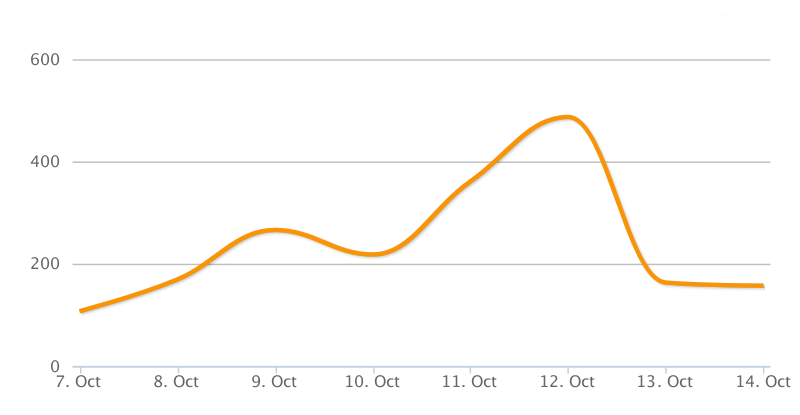
\includegraphics[width=1\linewidth]{Images/FirstSearch_QuantumComputing.png}
   \caption{} 
 \end{subfigure}

 \begin{subfigure}[t]{0.95\textwidth}
   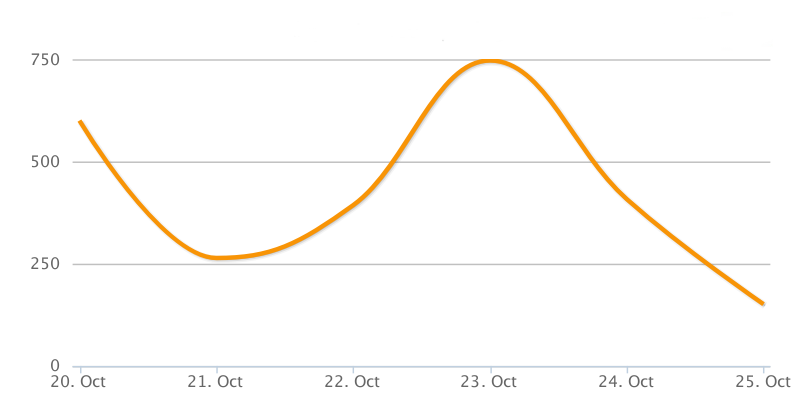
\includegraphics[width=1\linewidth]{Images/SecondSearch_QuantumComputing.png}
   \caption{}
 \end{subfigure}
 \caption{(a) Time distribution of the number of tweets with hashtag \#quantumcomputing posted between 7 and 14 October 2017. (b) As for (a) but over the time period between 20 and 25 October 2017.} 
 \label{First-SecondSearch_QuantumComputing}
\end{figure}

The distribution of the number of tweets mentioning the hashtag \#quantumcomputing over the considered time periods is shown in figure \ref{First-SecondSearch_QuantumComputing}. The plots indicate that, typically, \#quantumcomputing is mentioned in hundreds of tweets each day. The potential reach offered by \#quantumcomputing is available in table \ref{Summary_QuantumComputing}. This is calculated as the sum of the followers of the profiles which posted tweets mentioning the considered keywords. The table shows that \#quantumcomputing reaches a potential community of the order of ten million users in roughly a week.

\section{Monitoring of the HPC hashtag} \label{Monitoring_of_the_HPC_hashtag}
An analysis similar to the one outlined in section \ref{Monitoring_of_the_QT_hashtag} was conducted for the HPC case. The considered keyword was \#hpc. This hashtag was chosen as it identifies mentions to the general thematic area.

\begin{table}[t]
 \begin{center}
  \begin{tabular}{cccc}
   \hline 
   \hline
   Time period & Tweets & Users & Potential Reach \\ 
   \hline
   \hline
   4 - 14 Oct 2017 & 2 857 & 1 372 & 11 533 160  \\
   20 - 25 Oct 2017 & 3 015 & 1 475 & 13 315 746  \\
   \hline
   \hline
  \end{tabular}
 \end{center} 
 \caption{Statistics calculated for the mentions on Twitter of the hashtag \#hpc over the monitored time periods. The potential reach is defined as the total aggregate number of followers of the accounts which mentioned the considered keyword in their tweets.}
\label{Summary_HPC} 
\end{table}

\begin{figure}
 \centering
 \begin{subfigure}[b]{0.95\textwidth}
   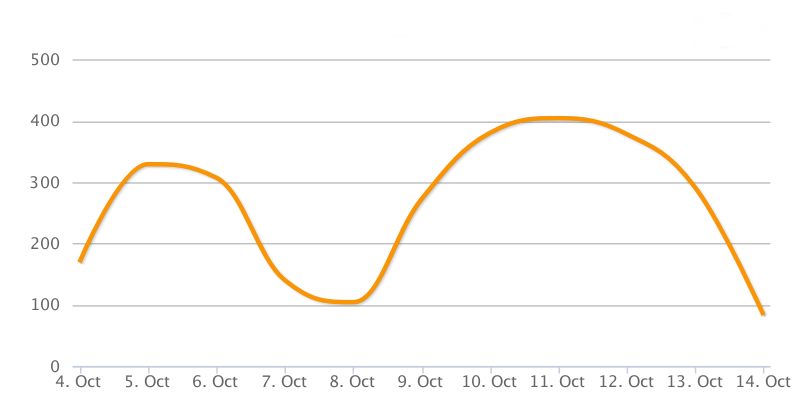
\includegraphics[width=1\linewidth]{Images/FirstSearch_HPC.png}
   \caption{} 
 \end{subfigure}

 \begin{subfigure}[b]{0.95\textwidth}
   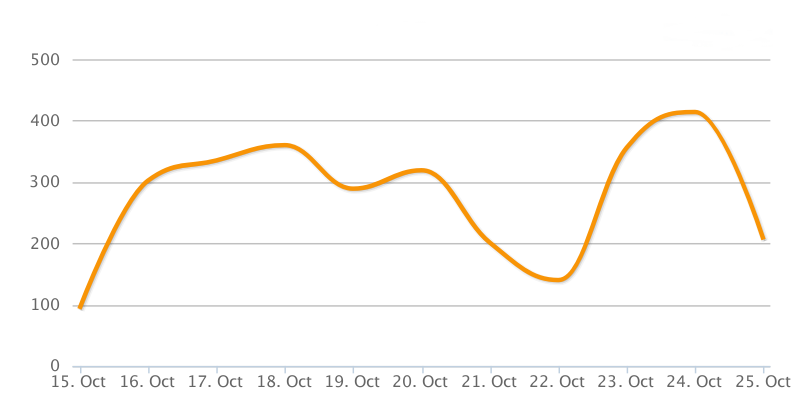
\includegraphics[width=1\linewidth]{Images/SecondSearch_HPC.png}
   \caption{}
 \end{subfigure}
 \caption{(a) Time distribution of the number of tweets with hashtag \#hpc posted between 4 and 14 October 2017. (b) As for (a) but over the time period between 15 and 25 October 2017.} 
 \label{First-SecondSearch_HPC}
\end{figure}

\begin{figure}
 \centering
 \begin{subfigure}[b]{0.95\textwidth}
   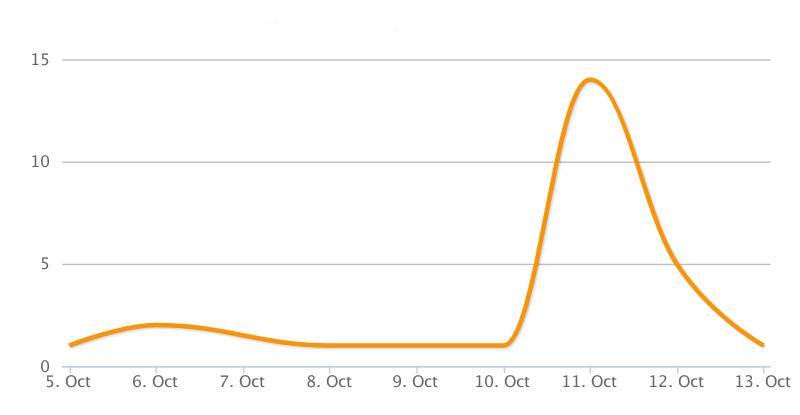
\includegraphics[width=1\linewidth]{Images/FirstSearch_HPC-QuantumComputing.png}
   \caption{} 
 \end{subfigure}

 \begin{subfigure}[b]{0.95\textwidth}
   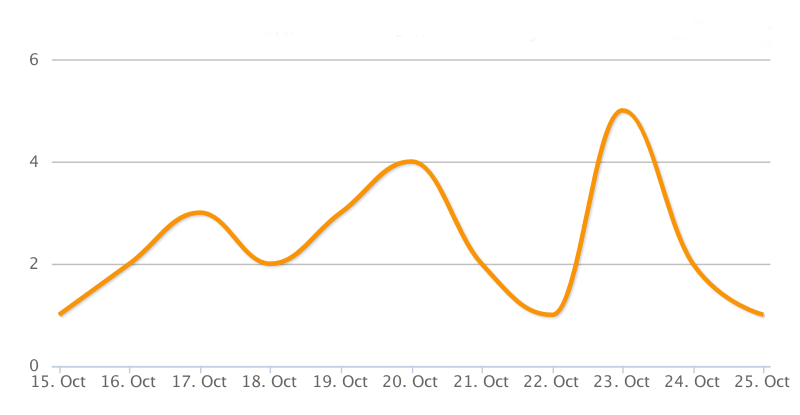
\includegraphics[width=1\linewidth]{Images/SecondSearch_HPC-QuantumComputing.png}
   \caption{}
 \end{subfigure}
 \caption{(a) Time distribution of the number of tweets with hashtags \#hpc and \#quantumcomputing posted between 5 and 13 October 2017. (b) As for (a) but over the time period between 15 and 25 October 2017.} 
 \label{First-SecondSearch_HPC-QuantumComputing}
\end{figure}

The monitored time periods ranged from 4 to 14 and from 15 to 25 October 2017. The time distributions of the tweets mentioning \#hpc are shown in figure \ref{First-SecondSearch_HPC}. The plots indicate that \#hpc is mentioned in hundreds of tweets per day.

An overview of the potential reach achievable with \#hpc is available in Table \ref{Summary_HPC}. Similarly to \#quantumcomputing, the potential reach of \#hpc is of the order of ten million of users over roughly a week. 

\section{Comparison of the results} \label{Comparison_of_the_results}
The monitoring activities outlined in sections \ref{Monitoring_of_the_QT_hashtag} and \ref{Monitoring_of_the_HPC_hashtag} suggest the following:

\begin{itemize}
 \item Tweets on QTs have a potential reach of millions of people via Twitter. Thus, it may be worth for FET QT projects to consider Twitter as a suitable channel for communication and dissemination activities.
 \item The potential reaches of tweets mentioning \#quantumcomputing and \#hpc share the same order of magnitude. The same holds for the total amount of tweets and users. Hence, QT projects may achieve results similar to those reported in chapter \ref{HPC_projects_on_Twitter} for the case of HPC initiatives. 
\end{itemize}

It is worth noting that the number of tracked posts mentioning both hashtags is very low, as suggested in figure \ref{First-SecondSearch_HPC-QuantumComputing}. The plots show that the amount of tweets is one order of magnitude smaller than those in figures \ref{First-SecondSearch_QuantumComputing} and \ref{First-SecondSearch_HPC}. The result is probably due to the fact that QTs and HPC pursue different strategies to improve current computers, see section \ref{Online_presence_breakdown}. As a consequence, QT projects may generate an amount of conversations on FET-funded research comparable to that provided by HPC initiatives. 

\section{Chapter summary} 
In this chapter, the following items have been discussed: 

\begin{enumerate}
 \item FET QT projects are not active on Twitter. Nevertheless, an estimate of their potential reach indicates a community of millions of profiles. This suggests that it may be worth for QT projects to consider Twitter for developing effective communication and dissemination strategies.
 \item The potential reach of QT and HPC projects on Twitter were assessed to be comparable. Moreover, conversations on both topics are very rare. Hence, the development of communication campaigns making use of Twitter may enable QT projects to increase the spread of FET-funded research by the same factor as HPC initiatives.         
\end{enumerate}